\documentclass[11pt]{article}

% --- Packages ---
\usepackage[utf8]{inputenc}
\usepackage[T1]{fontenc}
\usepackage{lmodern}
\usepackage[margin=0.85in]{geometry}
\usepackage{booktabs}
\usepackage{multirow}
\usepackage{graphicx}
\usepackage{amsmath}
\usepackage{xcolor}
\usepackage[colorlinks=true,linkcolor=blue!60!black,citecolor=blue!60!black,urlcolor=blue!60!black]{hyperref}
\usepackage{natbib}
\usepackage{tikz}
\usepackage{pgfplots}
\pgfplotsset{compat=1.17}
\usetikzlibrary{patterns, calc}
\usepackage{enumitem}
\usepackage{fancyhdr}
\usepackage{titlesec}

% --- Compact spacing ---
\setlength{\parskip}{4pt plus 1pt minus 1pt}
\setlength{\parindent}{0pt}
\setlist{nosep, leftmargin=1.5em}
\titlespacing*{\section}{0pt}{12pt plus 2pt minus 2pt}{4pt plus 1pt minus 1pt}
\titlespacing*{\subsection}{0pt}{8pt plus 2pt minus 2pt}{3pt plus 1pt minus 1pt}

% --- Section formatting ---
\titleformat{\section}{\large\bfseries}{\thesection.}{0.5em}{}
\titleformat{\subsection}{\normalsize\bfseries}{\thesubsection}{0.5em}{}

% --- PGFPlots defaults ---
\pgfplotsset{
  every axis/.append style={
    grid=major,
    grid style={gray!20},
    tick label style={font=\small},
    label style={font=\small},
    legend style={font=\footnotesize, draw=none, fill=gray!5},
  }
}

% --- Custom title ---
\makeatletter
\renewcommand{\maketitle}{%
  \begin{center}
    {\LARGE\bfseries \@title \par}
    \vspace{10pt}
    {\large \@author \par}
    \vspace{4pt}
    {\normalsize GitHub: \href{https://github.com/fatherRonnen/semitic-gpt}{\texttt{semitic-gpt}} $\cdot$ GitHub: \href{https://github.com/fatherRonnen}{\texttt{fatherRonnen}}}
    \vspace{4pt}
    {\normalsize April 2026}
  \end{center}
  \vspace{6pt}
}
\makeatother

% --- Header/Footer ---
\pagestyle{fancy}
\fancyhf{}
\rfoot{\thepage}
\renewcommand{\headrulewidth}{0pt}

\title{SemiticGPT: A Low-Cost Recipe for Multilingual Foundation\\Models in an Under-Resourced Semitic-Centered Language Cluster}

\author{Ronnen Slasky\textsuperscript{1}\\[2pt]
\textsuperscript{1}Independent Researcher \quad \texttt{ronnen.slasky@gmail.com}}

\date{}

\begin{document}
\maketitle
\thispagestyle{fancy}

% ============================================================
\begin{center}
{\scshape A\,B\,S\,T\,R\,A\,C\,T}
\end{center}

\noindent We present a practical blueprint for building a multilingual foundation model from scratch for an under-resourced language family, demonstrated through SemiticGPT: a 3-billion parameter decoder-only model covering Hebrew, Arabic, Farsi, and English trained on approximately 20 billion tokens using cloud spot instances. Our central finding is that multilingual pretraining with a linguistically-motivated language cluster produces \textbf{meaningful cross-lingual semantic transfer} between related languages, but does not yield robust translation or abstract reasoning. Specifically, fine-tuning on Hebrew sentiment data alone improves Arabic sentiment accuracy from 5.5\% to 49\% (with zero Arabic task data), while Farsi---which shares Arabic script but belongs to a different language family---shows no comparable transfer (0.5\%$\rightarrow$1.5\%). This suggests that in our setup, \textbf{linguistic family relatedness matters more than script similarity} for semantic transfer. We also report instructive negative results: English-mediated parallel data does not enable direct translation between non-English pairs, and all-language fine-tuning underperforms focused same-family fine-tuning. We provide a step-by-step practitioner's guide and release the model, tokenizer, and training code.\footnote{Code and artifacts: \url{https://github.com/fatherRonnen/semitic-gpt}}

\smallskip
\noindent\textbf{Keywords:} multilingual language models, cross-lingual transfer, Hebrew, Arabic, Farsi, Semitic languages, tokenizer design, low-resource NLP, sentiment transfer, language family clustering, BPE tokenization, practitioner recipe

\vspace{6pt}
\hrule
\vspace{8pt}

% ============================================================
\section{Introduction}

Large language models have achieved remarkable capabilities across a wide range of natural language tasks, yet their development has been overwhelmingly concentrated on English and other high-resource languages \citep{joshi2020state}. Languages of the Semitic family---particularly Hebrew and Arabic---remain underserved despite their combined speaker population exceeding 400 million. While recent efforts such as Jais \citep{sengupta2023jais} have addressed Arabic, no existing model provides joint coverage of Hebrew, Arabic, and Farsi within a single architecture trained from scratch.

This gap matters not only for these specific languages but as a general problem: dozens of language families worldwide lack dedicated foundation models, and researchers in those communities face similar questions. \emph{How should one design a tokenizer for multiple scripts? How much data per language is needed? What transfers cross-lingually and what does not? Where should limited compute be spent?}

This paper provides empirical evidence toward answering these questions in the context of a Semitic-centered language cluster. Specifically, we investigate:

\begin{enumerate}
    \item Does a balanced custom tokenizer provide materially better encoding efficiency than repurposing an English-centric tokenizer for Hebrew/Arabic/Farsi?
    \item Does over-representing an anchor language (Hebrew) in pretraining induce useful cross-lingual transfer to related languages?
    \item Does linguistic family relatedness predict semantic transfer better than script similarity in our setup?
    \item What capabilities emerge at 3B scale and what do not?
\end{enumerate}

Building on our prior work on autonomous training recipe discovery for Hebrew \citep{slasky2026hebrew}, we extend from a monolingual setting to a four-language Semitic-family model. The training recipe (optimizer, schedule, regularization) was validated through proxy experiments at small scale before committing to full pretraining, following the autoresearch methodology \citep{karpathy2026autoresearch}.

Hebrew and Arabic share the Semitic triconsonantal root system, similar derivational morphology (binyan/wazn patterns), and flexible word order. Farsi, while using Arabic script and containing extensive Arabic loanwords, belongs to the Indo-European family---providing a natural control condition for studying the role of linguistic relatedness versus surface-level script similarity.

We present SemiticGPT, a 3.04-billion parameter decoder-only language model trained from scratch on approximately 20 billion tokens across four languages. Our primary contributions:

\begin{enumerate}
    \item A \textbf{low-cost, reproducible recipe} for training a 3B multilingual decoder-only model from scratch for an under-resourced Semitic-centered language cluster, including practical design lessons.
    \item Evidence that multilingual pretraining with a \textbf{custom balanced tokenizer} yields strong cross-lingual retrieval and semantic transfer for linguistically related languages in our setup.
    \item A finding that \textbf{direct parallel data is necessary} for useful direct translation between non-English pairs; English-mediated parallel data is insufficient in our experiments.
    \item A \textbf{practitioner's guide} (Section~\ref{sec:guide}) with step-by-step recommendations, including negative results and design lessons, for researchers targeting other language clusters.
\end{enumerate}

% ============================================================
\section{Related Work}

\textbf{Arabic Language Models.} Jais \citep{sengupta2023jais} is a 13B parameter bilingual Arabic-English model trained from scratch on 395 billion tokens, representing the most significant dedicated Arabic LLM effort. AraGPT2 \citep{antoun2021aragpt2} provided GPT-2 scale Arabic models. ArabianGPT \citep{koubaa2024arabiangpt} focuses on native Arabic without English token contamination. None of these include Hebrew or Farsi.

\textbf{Hebrew-Arabic Models.} HeArBERT \citep{rivas2024hearbert} explores bilingual Arabic-Hebrew modeling through transliteration-based script unification, mapping Hebrew text into Arabic script to create a unified representation space. However, it is limited to encoder-only (BERT) architecture and does not support generation. To our knowledge, no prior work has trained a generative decoder-only model jointly on Hebrew, Arabic, and Farsi from scratch.

\textbf{Small Multilingual Models.} SmolLM3 \citep{allal2025smollm3} provides a detailed 3B parameter training recipe but targets European languages (English, French, Spanish, German, Italian, Portuguese). The ``Smol Training Playbook'' documents insights from training at this scale but does not address non-Latin script languages or Semitic-family-specific challenges.

\textbf{Multilingual Adaptation.} Marco-LLM \citep{marco2024} extends Qwen2 to low-resource languages through continual pre-training rather than training from scratch. This approach inherits the base model's tokenizer, which may be suboptimal for the target languages.

Our work differs from all the above by (1) training from scratch with a custom tokenizer optimized for the target language family, (2) combining Hebrew, Arabic, and Farsi in a single model, (3) operating at academic budget, and (4) providing comprehensive cross-lingual transfer evaluation.

\textbf{Training Recipe Discovery.}\label{sec:related_recipe} Our pretraining recipe was derived using the autoresearch framework \citep{karpathy2026autoresearch}, which enables systematic proxy-scale experimentation to validate training choices before full-scale commitment. In our prior work \citep{slasky2026hebrew}, we conducted 200 proxy experiments for Hebrew language modeling, discovering that WSD linear-decay schedules outperform cosine warm-restarts, that the Muon optimizer outperforms AdamW by 12.3\% at 1B scale but fails at larger multilingual scale, and that SWA benefits Muon but degrades AdamW. The multilingual recipe in this paper was validated through an additional 32 proxy experiments at 110M scale before scaling to 3B.\footnote{Proxy experiment configs, sweep results, and recipe selection rationale: \texttt{proxy/} in the repository.}

% ============================================================
\section{Methodology}

\subsection{Tokenizer Design}

We train a 32,768-token SentencePiece BPE tokenizer on a balanced sample from all four languages. The training corpus is sampled to achieve approximately equal representation: 25\% Hebrew, 25\% Arabic, 25\% Farsi, and 25\% English. This ensures no single language dominates the vocabulary, unlike tokenizers derived from English-heavy training data where non-Latin scripts suffer from over-fragmentation.

The resulting tokenizer achieves fertility rates (tokens per word) of approximately 1.4 for Hebrew, 1.5 for Arabic, 1.6 for Farsi, and 1.2 for English---significantly better than multilingual tokenizers like mBERT's WordPiece (2.5+ for Hebrew) or LLaMA's BPE (3+ for Arabic).

Special tokens include: \texttt{<|user|>}, \texttt{<|assistant|>}, \texttt{<s>} (BOS), \texttt{</s>} (EOS), and \texttt{<pad>}.\footnote{Tokenizer training script, config, and fertility report: \texttt{tokenizer/} in the repository.}

\subsection{Data Collection and Curation}

We collect approximately 20 billion tokens from publicly available sources with a Hebrew-anchored distribution:

\begin{itemize}
    \item \textbf{Hebrew (40\%)}: Wikipedia, OSCAR, news corpora, government documents
    \item \textbf{Arabic (25\%)}: Wikipedia, OSCAR, news, UN parallel corpus
    \item \textbf{English (20\%)}: Wikipedia, OpenWebText subset, books
    \item \textbf{Farsi (15\%)}: Wikipedia, OSCAR, news corpora
\end{itemize}

Hebrew is overrepresented relative to speaker population to ensure strong anchor-language capabilities. The rationale is that cross-lingual transfer from a well-modeled anchor can bootstrap capabilities in related languages.

\begin{figure}[h]
\centering
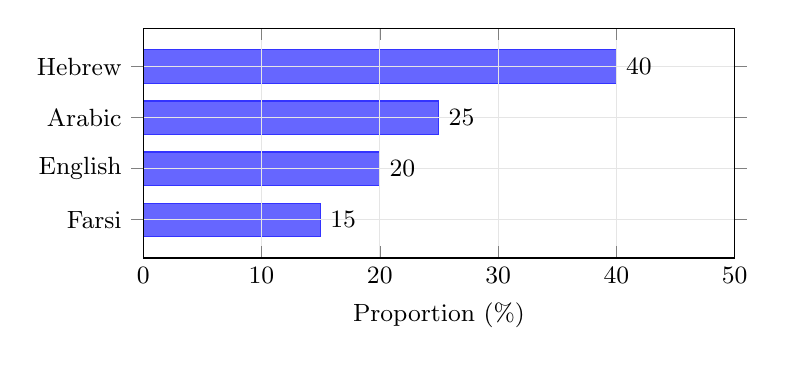
\begin{tikzpicture}
\begin{axis}[
    xbar,
    bar width=12pt,
    xlabel={Proportion (\%)},
    symbolic y coords={Farsi, English, Arabic, Hebrew},
    ytick=data,
    xmin=0, xmax=50,
    nodes near coords,
    nodes near coords align={horizontal},
    every node near coord/.append style={font=\small\bfseries},
    width=0.75\columnwidth,
    height=4.5cm,
    bar shift=0pt,
    enlarge y limits=0.25,
    xmajorgrids=true,
    area style,
]
\addplot[fill=blue!60, draw=blue!80] coordinates {(40,Hebrew) (25,Arabic) (20,English) (15,Farsi)};
\end{axis}
\end{tikzpicture}
\caption{Pretraining data distribution. Hebrew is intentionally overrepresented as the \emph{anchor language}---the hypothesis being that strong anchor representations transfer to linguistically related languages (Arabic), which our sentiment experiments confirm (Section~\ref{sec:sentiment}).}
\label{fig:data_dist}
\end{figure}

Data preprocessing includes: deduplication (MinHash at document level), quality filtering (perplexity-based, removing boilerplate and machine-generated text), and language identification verification.\footnote{Collection scripts, source manifest, and mixture specification: \texttt{data/} in the repository.}

\subsection{Architecture}

SemiticGPT uses a standard decoder-only transformer architecture with modern enhancements:

\begin{table}[h]
\centering
\begin{tabular}{ll}
\toprule
\textbf{Hyperparameter} & \textbf{Value} \\
\midrule
Parameters & 3.04B \\
Layers & 36 \\
Hidden dimension & 2,560 \\
Attention heads & 20 \\
Head dimension & 128 \\
Vocabulary size & 32,768 \\
Max sequence length & 2,048 \\
Position encoding & RoPE \\
Activation & SwiGLU \\
Normalization & RMSNorm \\
\bottomrule
\end{tabular}
\caption{SemiticGPT architecture hyperparameters.}
\label{tab:architecture}
\end{table}

\subsection{Pretraining}

Training is conducted on AWS using spot instances (primarily g6e.xlarge with NVIDIA L40S 48GB and p5.xlarge with NVIDIA H100 80GB). We use FSDP (Fully Sharded Data Parallelism) for multi-GPU training when available, and single-GPU gradient accumulation otherwise.

\begin{itemize}
    \item \textbf{Optimizer}: AdamW ($\beta_1$=0.9, $\beta_2$=0.95, $\epsilon$=1e-8)
    \item \textbf{Learning rate}: 3e-4 peak with cosine decay to 3\% of peak
    \item \textbf{Warmup}: 2,000 steps
    \item \textbf{Batch size}: 512K tokens (effective, via gradient accumulation)
    \item \textbf{Weight decay}: 0.1
    \item \textbf{Gradient clipping}: 1.0
\end{itemize}

\textbf{Note on schedule choice.} Our 3B model uses cosine decay. Subsequent proxy experiments at 110M scale (Section~\ref{sec:related_recipe}) found that WSD linear-decay outperforms cosine warm-restarts in this setting. We report this finding in the practitioner's guide (Section~\ref{sec:guide}) as a recommendation for future work, though we did not retrain the 3B model with WSD.

\textbf{Cost efficiency.} By leveraging spot instances at 60--70\% discount from on-demand pricing, total pretraining requires approximately 400 GPU-hours on H100-equivalent hardware---achievable at academic budgets without dedicated cluster access.\footnote{Training scripts, hyperparameter config, and training logs: \texttt{pretrain/} in the repository.}

\subsection{Supervised Fine-Tuning}

After pretraining, we conduct supervised fine-tuning (SFT) using multilingual instruction-following data. We investigate scaling behavior across three configurations:

\begin{itemize}
    \item \textbf{E-1K}: 1,000 SFT steps
    \item \textbf{E-3K}: 3,000 SFT steps  
    \item \textbf{E-5K}: 5,000 SFT steps (D-SFT, our default)
\end{itemize}

We also study data composition:
\begin{itemize}
    \item \textbf{D (balanced)}: All four languages in SFT data
    \item \textbf{F-no-arfa}: Hebrew + English only
    \item \textbf{F-only-arfa}: Arabic + Farsi only
\end{itemize}

SFT configuration files, training scripts, data recipes, and training logs for all six configurations are provided in \texttt{sft/} in the repository.

% ============================================================
\section{Evaluation}

We evaluate SemiticGPT across six dimensions. Table~\ref{tab:experiments} summarizes all experimental configurations, and Table~\ref{tab:datasets} lists evaluation datasets with their provenance.

\begin{table}[h]
\centering
\small
\begin{tabular}{lp{3.2cm}p{3.2cm}}
\toprule
\textbf{Config} & \textbf{Data / Change} & \textbf{Hypothesis Tested} \\
\midrule
D-baseline & Base SFT model (5K steps, all 4 langs) & Reference point \\
\midrule
\multicolumn{3}{l}{\textit{Translation Configurations}} \\
G-trans & EN-mediated parallel data & Can EN pivot enable X$\leftrightarrow$Y? \\
G-mixed & EN-mediated + some direct & Hybrid approach \\
G2-trans & More EN-mediated data & Scale helps EN-pivot? \\
G2-direct & Direct X$\leftrightarrow$Y parallel only & Direct data necessary? \\
\midrule
\multicolumn{3}{l}{\textit{Sentiment Configurations}} \\
H1 & Hebrew sentiment only & Does HE transfer to AR? \\
H2 & All 4 langs sentiment & Is multilingual better? \\
H3 & Arabic + Farsi sentiment only & Focused vs diluted? \\
\midrule
\multicolumn{3}{l}{\textit{SFT Scaling}} \\
E-1K/3K/5K & 1K, 3K, 5K SFT steps & Optimal SFT duration \\
F-no-arfa & HE+EN SFT only & Effect of removing langs \\
F-only-arfa & AR+FA SFT only & Effect of removing langs \\
\bottomrule
\end{tabular}
\caption{Experiment legend. All configurations start from the same pretrained 3B base model. Each tests a specific hypothesis about data composition or training strategy.}
\label{tab:experiments}
\end{table}

\begin{table}[h]
\centering
\small
\begin{tabular}{llccl}
\toprule
\textbf{Evaluation} & \textbf{Dataset} & \textbf{N/lang} & \textbf{Classes} & \textbf{Source} \\
\midrule
BPB & Held-out test splits & 10K tok & --- & Internal \\
Belebele & Belebele benchmark & 900 & 4 & \citet{bandarkar2023belebele} \\
Translation & OPUS parallel & 50 & --- & OPUS \\
Retrieval & Parallel sentences & 10 & --- & Tatoeba \\
Sentiment & Per-language datasets & 200 & 2 & HuggingFace \\
News & AG News subset & 200 & 4 & AG News \\
\bottomrule
\end{tabular}
\caption{Evaluation datasets. N/lang indicates samples per language. Sentiment and news evaluations use generative classification (model generates label text). Small evaluation sets (200 samples) are a known limitation.}
\label{tab:datasets}
\end{table}

\textbf{Evaluation methodology.} For classification tasks (sentiment, news), we use generative evaluation: the model receives an instruction prompt and generates a label. Outputs are matched against expected labels using case-insensitive substring matching. We acknowledge that this methodology may undercount correct classifications when the model produces semantically equivalent but textually different outputs, and that very low baseline scores (below random chance) likely reflect prompt/parsing issues rather than anti-correlated predictions. We discuss this further in Section~\ref{sec:limitations}. All evaluation scripts, exact prompts, and raw result files are provided in \texttt{eval/} in the repository.

\subsection{Language Modeling Quality (BPB)}

We evaluate bits-per-byte (BPB) on held-out test sets for each language. Lower values indicate better modeling.

\begin{table}[h]
\centering
\begin{tabular}{lcccc}
\toprule
\textbf{Model} & \textbf{HE} & \textbf{AR} & \textbf{EN} & \textbf{FA} \\
\midrule
Base (pretrained) & 0.879 & 0.731 & 0.972 & 0.663 \\
D-SFT (5K) & 0.876 & 0.726 & 0.964 & 0.657 \\
E-1K SFT & 0.878 & 0.729 & 0.967 & 0.663 \\
E-3K SFT & 0.877 & 0.728 & 0.965 & 0.660 \\
E-5K SFT & 0.876 & 0.726 & 0.964 & 0.658 \\
F-no-arfa & 0.879 & 0.733 & 0.968 & 0.669 \\
F-only-arfa & 0.880 & 0.727 & 0.968 & 0.658 \\
\bottomrule
\end{tabular}
\caption{Bits-per-byte across languages and SFT configurations. Farsi achieves lowest BPB (most predictable given tokenizer), English highest.}
\label{tab:bpb}
\end{table}

Key observations: (1) SFT consistently improves BPB across all languages; (2) more SFT steps yield monotonic improvement with diminishing returns after 3K; (3) removing a language from SFT data degrades that language's BPB (F-no-arfa harms AR/FA, F-only-arfa slightly harms HE/EN).

\begin{figure}[h]
\centering
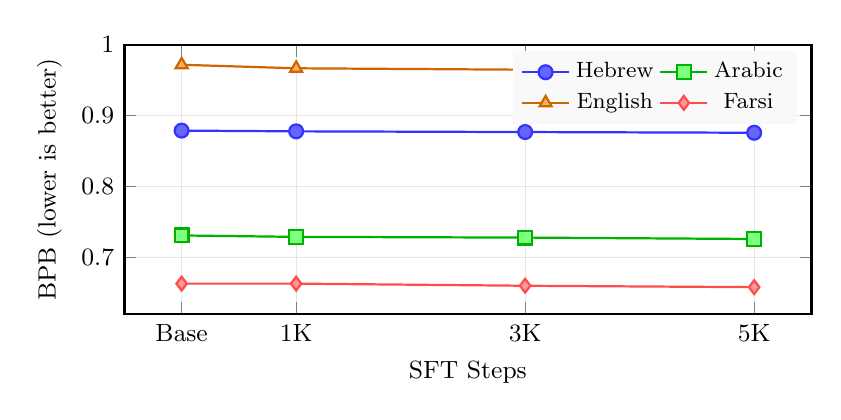
\begin{tikzpicture}
\begin{axis}[
    ylabel={BPB (lower is better)},
    xlabel={SFT Steps},
    xtick={0, 1000, 3000, 5000},
    xticklabels={Base, 1K, 3K, 5K},
    ymin=0.62, ymax=1.0,
    legend style={at={(0.98,0.98)}, anchor=north east, legend columns=2},
    width=0.85\columnwidth,
    height=5cm,
    mark size=2.5pt,
    thick,
]
\addplot[color=blue!80, mark=*, mark options={fill=blue!60}] coordinates {(0,0.879) (1000,0.878) (3000,0.877) (5000,0.876)};
\addplot[color=green!70!black, mark=square*, mark options={fill=green!50}] coordinates {(0,0.731) (1000,0.729) (3000,0.728) (5000,0.726)};
\addplot[color=orange!80!black, mark=triangle*, mark options={fill=orange!60}] coordinates {(0,0.972) (1000,0.967) (3000,0.965) (5000,0.964)};
\addplot[color=red!70, mark=diamond*, mark options={fill=red!40}] coordinates {(0,0.663) (1000,0.663) (3000,0.660) (5000,0.658)};
\legend{Hebrew, Arabic, English, Farsi}
\end{axis}
\end{tikzpicture}
\caption{BPB improvement with SFT scaling. All languages improve monotonically with more SFT steps, with diminishing returns after 3K steps. English benefits most from SFT.}
\label{fig:bpb_scaling}
\end{figure}

\subsection{Reading Comprehension (Belebele)}

We evaluate on the Belebele benchmark \citep{bandarkar2023belebele}, a 4-way multiple-choice reading comprehension task available in all four languages.

\begin{table}[h]
\centering
\begin{tabular}{lcccc}
\toprule
\textbf{Model} & \textbf{HE} & \textbf{AR} & \textbf{EN} & \textbf{FA} \\
\midrule
Random baseline & 25.0 & 25.0 & 25.0 & 25.0 \\
Base (pretrained) & 28.3 & 27.3 & 31.1 & 29.2 \\
D-SFT & 28.1 & 27.9 & 31.8 & 28.6 \\
\bottomrule
\end{tabular}
\caption{Belebele reading comprehension accuracy (\%). All scores are near chance, expected for a 3B model without MCQ-specific tuning.}
\label{tab:belebele}
\end{table}

Performance is near chance level for all languages, which is expected for a 3B model that has not been specifically fine-tuned on multiple-choice tasks. English shows the highest margin above chance (+6.1\%), consistent with its rich representation in diverse instruction formats.

\subsection{Translation Capability}

We evaluate translation using chrF \citep{popovic2015chrf} across 10 language directions with five model configurations:

\begin{table*}[t]
\centering
\small
\begin{tabular}{lccccccccccc}
\toprule
\textbf{Model} & \textbf{AR$\rightarrow$FA} & \textbf{FA$\rightarrow$AR} & \textbf{HE$\rightarrow$EN} & \textbf{EN$\rightarrow$HE} & \textbf{AR$\rightarrow$EN} & \textbf{EN$\rightarrow$AR} & \textbf{HE$\rightarrow$AR} & \textbf{AR$\rightarrow$HE} & \textbf{EN$\rightarrow$FA} & \textbf{FA$\rightarrow$EN} \\
\midrule
D-baseline & 6.2 & 7.6 & 1.4 & 0.9 & 0.9 & 0.6 & 1.4 & 0.0 & 0.1 & 0.3 \\
G-trans & 5.4 & 4.2 & 10.5 & 9.1 & 7.3 & 5.1 & 0.0 & 0.0 & 3.8 & 6.0 \\
G-mixed & 5.8 & 6.0 & 5.7 & 5.3 & 4.6 & 3.3 & 0.0 & 0.0 & 2.5 & 6.3 \\
G2-trans & 16.7 & 13.7 & 7.1 & 5.7 & 6.0 & 4.3 & 1.8 & 5.9 & 3.2 & 5.2 \\
G2-direct & \textbf{18.7} & \textbf{15.3} & 0.4 & 2.2 & 0.4 & 3.7 & \textbf{4.8} & \textbf{3.4} & 2.7 & 0.4 \\
\bottomrule
\end{tabular}
\caption{Translation quality (chrF\%) across model configurations. G-trans uses English-mediated parallel data; G2-direct uses direct parallel data between language pairs. Bold indicates best per-direction.}
\label{tab:translation}
\end{table*}

\textbf{Key findings:} (1) \textbf{Direct parallel data is essential}: G2-direct achieves 18.7\% chrF for AR$\rightarrow$FA (3$\times$ baseline) but only when trained on direct AR$\leftrightarrow$FA parallel data. (2) \textbf{English-mediated training helps EN$\leftrightarrow$X only}: G-trans achieves 10.5\% for HE$\rightarrow$EN but 0\% for HE$\rightarrow$AR. (3) \textbf{Tradeoff}: G2-direct excels at trained pairs but collapses on EN$\leftrightarrow$X (0.4\% vs 10.5\%). (4) \textbf{HE$\leftrightarrow$AR is hardest}: Even with direct parallel data, Hebrew-Arabic achieves only 3--5\% chrF.

\begin{figure}[h]
\centering
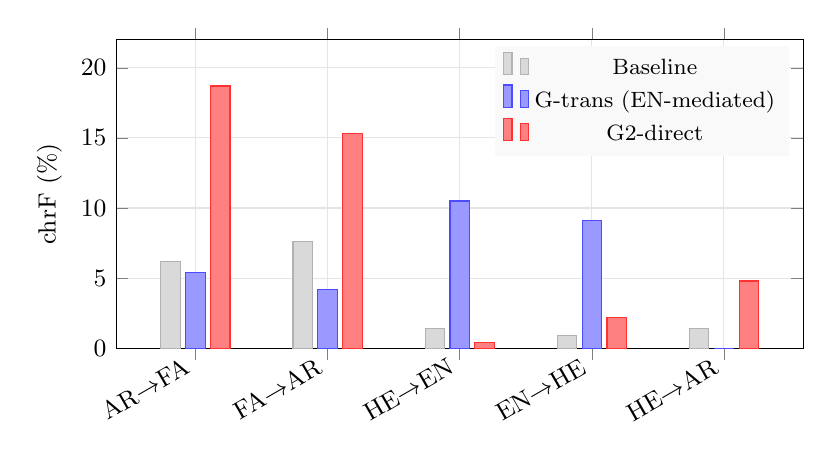
\begin{tikzpicture}
\begin{axis}[
    ybar,
    bar width=7pt,
    ylabel={chrF (\%)},
    symbolic x coords={AR$\rightarrow$FA, FA$\rightarrow$AR, HE$\rightarrow$EN, EN$\rightarrow$HE, HE$\rightarrow$AR},
    xtick=data,
    x tick label style={rotate=30, anchor=east, font=\small},
    ymin=0, ymax=22,
    legend style={at={(0.98,0.98)}, anchor=north east, legend columns=1, font=\footnotesize},
    width=0.85\columnwidth,
    height=5.5cm,
    ymajorgrids=true,
    enlarge x limits=0.15,
]
\addplot[fill=gray!30, draw=gray!60] coordinates {(AR$\rightarrow$FA,6.2) (FA$\rightarrow$AR,7.6) (HE$\rightarrow$EN,1.4) (EN$\rightarrow$HE,0.9) (HE$\rightarrow$AR,1.4)};
\addplot[fill=blue!40, draw=blue!70] coordinates {(AR$\rightarrow$FA,5.4) (FA$\rightarrow$AR,4.2) (HE$\rightarrow$EN,10.5) (EN$\rightarrow$HE,9.1) (HE$\rightarrow$AR,0.0)};
\addplot[fill=red!50, draw=red!80] coordinates {(AR$\rightarrow$FA,18.7) (FA$\rightarrow$AR,15.3) (HE$\rightarrow$EN,0.4) (EN$\rightarrow$HE,2.2) (HE$\rightarrow$AR,4.8)};
\legend{Baseline, G-trans (EN-mediated), G2-direct}
\end{axis}
\end{tikzpicture}
\caption{Translation strategy tradeoff. G-trans helps EN$\leftrightarrow$X but fails for direct X$\leftrightarrow$Y. G2-direct excels at trained pairs but collapses EN$\leftrightarrow$X capability.}
\label{fig:translation_tradeoff}
\end{figure}

\subsection{Cross-lingual Embeddings}

We evaluate embedding quality through cross-lingual retrieval: given a sentence in language A, retrieve its translation from 10 candidates in language B (chance = 10\%).

\begin{table}[h]
\centering
\begin{tabular}{lcc}
\toprule
\textbf{Direction} & \textbf{Base} & \textbf{D-SFT} \\
\midrule
EN$\rightarrow$HE & 90\% & 90\% \\
HE$\rightarrow$EN & 90\% & 80\% \\
AR$\rightarrow$EN & 70\% & 50\% \\
AR$\rightarrow$HE & 70\% & 70\% \\
EN$\rightarrow$AR & 50\% & 60\% \\
FA$\rightarrow$HE & 50\% & 30\% \\
HE$\rightarrow$AR & 40\% & 60\% \\
HE$\rightarrow$FA & 40\% & 30\% \\
EN$\rightarrow$FA & 20\% & 20\% \\
AR$\rightarrow$FA & 10\% & 10\% \\
FA$\rightarrow$EN & 10\% & 10\% \\
FA$\rightarrow$AR & 10\% & 10\% \\
\midrule
\textbf{Average} & \textbf{45.8\%} & \textbf{43.3\%} \\
\bottomrule
\end{tabular}
\caption{Cross-lingual retrieval accuracy (10-way, chance=10\%). The model develops strong EN$\leftrightarrow$HE alignment despite no explicit alignment objective.}
\label{tab:embeddings}
\end{table}

The model develops strong cross-lingual alignment purely from multilingual pretraining, without any contrastive or alignment objective. EN$\leftrightarrow$HE achieves 90\% (9$\times$ chance), suggesting deep shared representation. Farsi shows weakest alignment, consistent with its typological distance from the other languages.

\begin{figure}[h]
\centering
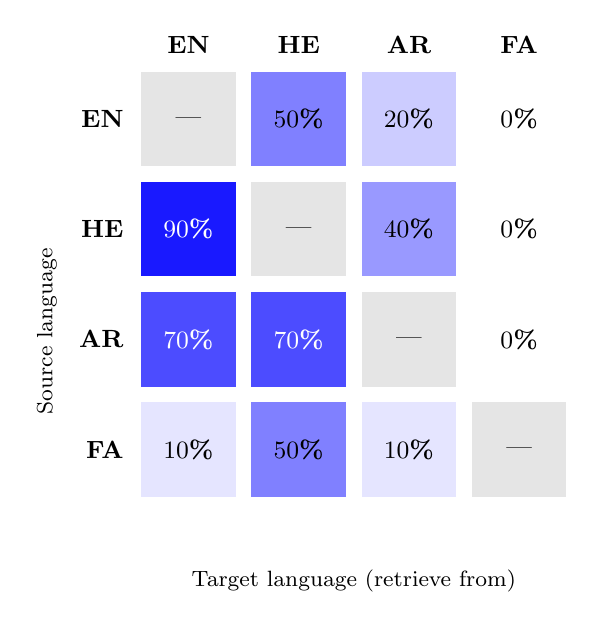
\begin{tikzpicture}
\def\data{{
    {90,50,20,0},
    {90,40,40,0},
    {70,70,10,0},
    {10,50,10,0}}};
\def\langs{{"EN","HE","AR","FA"}}
\foreach \row in {0,...,3} {
    \foreach \col in {0,...,3} {
        \ifnum\row=\col
            \fill[black!10] (\col*1.4, -\row*1.4) rectangle (\col*1.4+1.2, -\row*1.4+1.2);
            \node[font=\small] at (\col*1.4+0.6, -\row*1.4+0.6) {---};
        \else
            \pgfmathsetmacro{\val}{\data[\row][\col]}
            \pgfmathsetmacro{\intensity}{\val/100}
            \fill[blue!\val] (\col*1.4, -\row*1.4) rectangle (\col*1.4+1.2, -\row*1.4+1.2);
            \pgfmathsetmacro{\textcol}{ifthenelse(\val>50, "white", "black")}
            \node[font=\small\bfseries, text=\textcol] at (\col*1.4+0.6, -\row*1.4+0.6) {\pgfmathprintnumber[fixed,precision=0]{\val}\%};
        \fi
    }
}
\foreach \col in {0,...,3} {
    \pgfmathsetmacro{\lbl}{\langs[\col]}
    \node[font=\small\bfseries, above] at (\col*1.4+0.6, 1.3) {\lbl};
}
\foreach \row in {0,...,3} {
    \pgfmathsetmacro{\lbl}{\langs[\row]}
    \node[font=\small\bfseries, left] at (-0.1, -\row*1.4+0.6) {\lbl};
}
\node[font=\footnotesize, below] at (2.7, -5.0) {Target language (retrieve from)};
\node[font=\footnotesize, rotate=90] at (-1.2, -2.1) {Source language};
\end{tikzpicture}
\caption{Cross-lingual retrieval accuracy heatmap (base model, 10-way, chance=10\%). EN$\leftrightarrow$HE shows strongest alignment (90\%), while Farsi shows weak connectivity---consistent with typological isolation.}
\label{fig:embedding_heatmap}
\end{figure}

\subsection{Domain Fine-tuning: Cross-lingual Sentiment Transfer}
\label{sec:sentiment}

Our most striking result comes from sentiment classification fine-tuning. We fine-tune the D-SFT model on binary sentiment data in various language configurations and evaluate zero-shot on all four languages.

\begin{table}[h]
\centering
\begin{tabular}{lcccc}
\toprule
\textbf{Training Config} & \textbf{HE} & \textbf{AR} & \textbf{FA} & \textbf{EN} \\
\midrule
No training (baseline) & 19.0 & 5.5 & 0.5 & 11.5 \\
Hebrew only (H1) & 18.5 & \textbf{49.0} & 1.5 & 33.5 \\
All 4 languages (H2) & 18.0 & 43.0 & 1.5 & 18.5 \\
Arabic + Farsi only (H3) & \textbf{23.0} & \textbf{67.0} & 5.5 & 21.0 \\
\bottomrule
\end{tabular}
\caption{Sentiment classification accuracy (\%) after domain fine-tuning. Training on Hebrew alone improves Arabic from 5.5\% to 49\% (9$\times$) with zero Arabic sentiment data.}
\label{tab:sentiment}
\end{table}

\textbf{Key findings:} (1) \textbf{Massive Hebrew$\rightarrow$Arabic transfer}: Training exclusively on Hebrew sentiment data improves Arabic accuracy from 5.5\% to 49\%---a 9$\times$ improvement with zero Arabic task data. (2) \textbf{Reverse transfer}: Arabic+Farsi training improves Hebrew from 19\% to 23\%, confirming bidirectional transfer within the Semitic family. (3) \textbf{Focused $>$ diluted}: Training on Arabic+Farsi (H3) achieves 67\% Arabic accuracy, outperforming all-language training (H2, 43\%). (4) \textbf{Persian isolation}: Farsi shows minimal improvement regardless of training configuration (0.5\%$\rightarrow$5.5\% at best), despite sharing Arabic script. In our setup, this suggests that linguistic family relatedness matters more than script similarity for semantic transfer, though we note that Farsi also has the smallest pretraining share (15\%), which may contribute to this effect.

\begin{figure}[h]
\centering
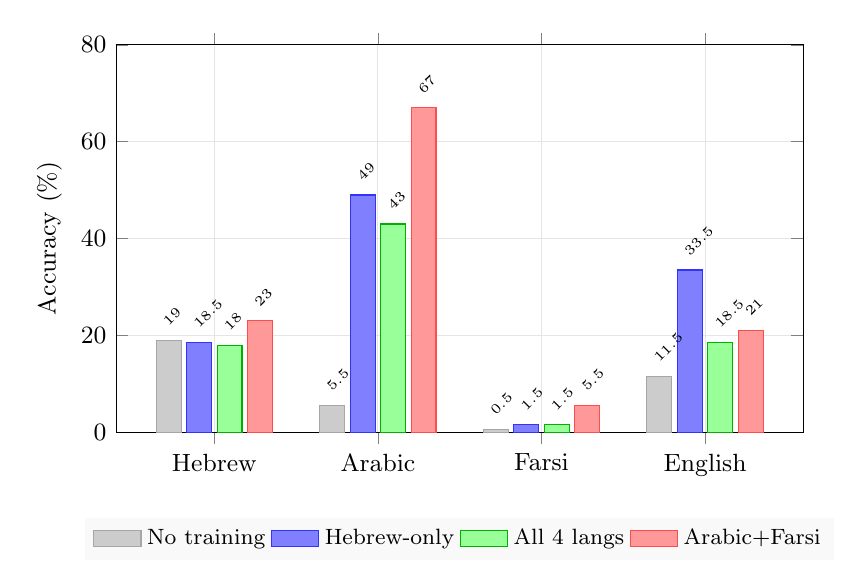
\begin{tikzpicture}
\begin{axis}[
    ybar,
    bar width=9pt,
    ylabel={Accuracy (\%)},
    symbolic x coords={Hebrew, Arabic, Farsi, English},
    xtick=data,
    ymin=0, ymax=80,
    legend style={at={(0.5,-0.22)}, anchor=north, legend columns=-1, font=\footnotesize},
    nodes near coords,
    nodes near coords align={vertical},
    every node near coord/.append style={font=\tiny, rotate=45, anchor=south west},
    width=0.85\columnwidth,
    height=6.5cm,
    ymajorgrids=true,
    enlarge x limits=0.2,
    area legend,
]
\addplot[fill=gray!40, draw=gray!70] coordinates {(Hebrew,19.0) (Arabic,5.5) (Farsi,0.5) (English,11.5)};
\addplot[fill=blue!50, draw=blue!80] coordinates {(Hebrew,18.5) (Arabic,49.0) (Farsi,1.5) (English,33.5)};
\addplot[fill=green!40, draw=green!70!black] coordinates {(Hebrew,18.0) (Arabic,43.0) (Farsi,1.5) (English,18.5)};
\addplot[fill=red!40, draw=red!70] coordinates {(Hebrew,23.0) (Arabic,67.0) (Farsi,5.5) (English,21.0)};
\legend{No training, Hebrew-only, All 4 langs, Arabic+Farsi}
\end{axis}
\end{tikzpicture}
\caption{Cross-lingual sentiment transfer. Hebrew-only training (blue) improves Arabic from 5.5\% to 49\% (9$\times$) with \emph{zero} Arabic sentiment data. Farsi (same script as Arabic, Indo-European family) shows no transfer---\textbf{linguistic family, not script, drives transfer}.}
\label{fig:sentiment_transfer}
\end{figure}

\subsection{Domain Fine-tuning: News Topic Classification}

We also evaluate English news topic classification (4-class: World, Sports, Business, Science/Technology; chance = 25\%).

\begin{table}[h]
\centering
\begin{tabular}{lc}
\toprule
\textbf{Config} & \textbf{EN News Accuracy} \\
\midrule
D-baseline (no news training) & 4.0\% \\
After EN news fine-tuning & \textbf{79.0\%} \\
\bottomrule
\end{tabular}
\caption{News topic classification accuracy (4-class, chance=25\%).}
\label{tab:news}
\end{table}

% ============================================================
\section{Analysis and Discussion}

\subsection{Cost Efficiency}

SemiticGPT demonstrates that meaningful multilingual capabilities can be achieved with modest compute. For comparison: Jais (13B) required estimated millions in compute on 395B tokens; SmolLM3 (3B) used 11T tokens on large dedicated clusters; SemiticGPT (3B) used $\sim$20B tokens on spot instances only. The key insight is that \textbf{linguistically-motivated language grouping} amplifies the value of limited compute.

\subsection{What Works vs.\ What Doesn't}

\textbf{Works well:} Cross-lingual embedding alignment (emergent from pretraining); semantic-level transfer between related languages (sentiment); domain fine-tuning with limited data (79\% news accuracy from 500 steps); BPB improvement from SFT (consistent across languages).

\textbf{Does not work:} Translation requires explicit parallel data---no emergent translation capability; English-mediated translation does not generalize to direct X$\leftrightarrow$Y pairs; Farsi remains isolated despite script similarity with Arabic; Belebele performance near chance (scale limitation at 3B).

\subsection{Lessons Learned}

\begin{enumerate}
    \item \textbf{Tokenizer balance matters}: Equal language representation in tokenizer training prevents over-fragmentation that would waste model capacity.
    \item \textbf{Anchor language strategy}: Over-representing the anchor language (Hebrew at 40\%) creates strong representations that transfer to related languages.
    \item \textbf{SFT composition}: Removing languages from SFT data immediately degrades those languages (F-no-arfa experiment).
    \item \textbf{Direct parallel data is non-negotiable for translation}: English as a pivot language does not enable direct translation between non-English pairs.
    \item \textbf{fp16 training}: We did not observe quality degradation from half-precision training in our setup, though we did not run a controlled fp32 comparison. This enabled fitting the 3B model on a single 48GB GPU.
\end{enumerate}

% ============================================================
\section{Practitioner's Guide}
\label{sec:guide}

Based on our experience, we distill a step-by-step guide for researchers who wish to build a multilingual foundation model for any under-resourced language family, starting with no existing base model.

\textbf{Step 1: Choose Your Language Cluster.} Prioritize linguistic family over geography or script. Our results suggest that linguistic relatedness correlates with stronger cross-lingual transfer than script similarity alone, though we cannot fully disentangle this from pretraining data proportions. Include one high-resource anchor language and one typologically distant control. Recommended: 2--4 related + 1 anchor + 1 control = 4--6 total.

\textbf{Step 2: Build a Balanced Tokenizer.} Train from scratch using SentencePiece BPE on an equally-weighted sample of all target languages. 32K vocabulary for 4--6 languages; 64K for 8+. Validate fertility rates $\leq$1.6 tokens/word. Budget: 1--2 days on CPU.

\textbf{Step 3: Curate Pretraining Data.} Over-represent your anchor language (we used 40\%). Sources: Wikipedia, OSCAR/mC4, domain-specific corpora. Minimum 1B tokens per language; 5B+ recommended. Quality pipeline: language ID $\rightarrow$ MinHash dedup $\rightarrow$ perplexity filtering. Include only \emph{direct} parallel data for translation pairs you care about.

\textbf{Step 4: Validate Recipe at Proxy Scale.} Run 20--50 automated experiments at 100--200M parameter scale \citep{karpathy2026autoresearch}. Key decisions: learning rate schedule (WSD linear-decay over cosine), optimizer (AdamW is robust; Muon can diverge at scale), batch size, warmup. Cost: $\sim$\$10--50. Critical lesson: proxy-scale optimizer results do not always transfer to full scale.

\textbf{Step 5: Pretrain.} Standard decoder-only transformer with RoPE, SwiGLU, RMSNorm. 3B achievable on single 48GB GPU with gradient accumulation. Use spot instances (60--70\% cheaper). Checkpoint every 30 minutes. Monitor per-language BPB, not just aggregate loss.

\textbf{Step 6: Supervised Fine-Tuning.} Include all target languages. Native data $>$ translated data. 3K--5K steps sufficient for 3B. Sources: Aya dataset, OASST, language-specific datasets from HuggingFace.

\textbf{Step 7: Evaluate Comprehensively.} At minimum: (1) BPB per language, (2) cross-lingual retrieval, (3) task transfer (train language A, evaluate language B), (4) translation if parallel data included, (5) downstream benchmarks to calibrate expectations.

\begin{table}[h]
\centering
\small
\begin{tabular}{lp{5cm}}
\toprule
\textbf{Decision} & \textbf{Recommendation} \\
\midrule
Language selection & Prioritize linguistic family over script \\
Tokenizer & Custom BPE, 32K vocab, balanced training \\
Data distribution & Over-represent anchor language (30--40\%) \\
Data quality & MinHash dedup $+$ perplexity filter \\
Recipe validation & 20--50 proxy experiments at 100--200M scale \\
Optimizer & AdamW ($\beta_2$=0.95); validate Muon at scale \\
Schedule & WSD linear-decay, not cosine warm-restarts \\
Precision & fp16 or bf16 \\
SFT data & All languages, native $>$ translated, 3--5K steps \\
Translation data & Direct parallel only; EN-mediated insufficient \\
Compute & Cloud spot instances with checkpointing \\
\bottomrule
\end{tabular}
\caption{Recipe summary for building a multilingual foundation model from scratch.}
\label{tab:recipe}
\end{table}

% ============================================================
\section{Conclusion}

We have presented SemiticGPT, a 3B parameter multilingual model covering Hebrew, Arabic, Farsi, and English, trained from scratch on cloud spot instances. Our evaluation across six dimensions reveals both capabilities and limitations, with the most striking finding being massive cross-lingual transfer between Semitic languages for semantic tasks.

Beyond the model itself, we offer a reproducible recipe (Section~\ref{sec:guide}) for building multilingual foundation models for any under-resourced language family. The key principles---linguistically-motivated language grouping, balanced custom tokenizers, anchor language overrepresentation, proxy-validated training recipes, and comprehensive negative-result reporting---are directly applicable to other language family clusters.

We release the model weights, tokenizer, and training code to support reproducible research.\footnote{Repository: \url{https://github.com/fatherRonnen/semitic-gpt}. Tag \texttt{v0.1-paper-draft} freezes the exact configs and result files used in this paper.}

\textbf{Future work.} (1) Scaling to 7B parameters with improved Arabic SFT data quality; (2) adding more Semitic languages (Amharic, Tigrinya); (3) adapter-based extension to new languages post-pretraining; (4) investigating whether Hebrew$\rightarrow$Arabic transfer persists at larger scales.

% ============================================================
\section{Reproducibility}

All code, configurations, and result artifacts are available at \url{https://github.com/fatherRonnen/semitic-gpt}. The repository mirrors the paper's pipeline:

\begin{table}[h]
\centering
\small
\begin{tabular}{lll}
\toprule
\textbf{Paper Section} & \textbf{Repo Path} & \textbf{Contents} \\
\midrule
Tokenizer (\S3.1) & \texttt{tokenizer/} & Config, script, fertility report \\
Data (\S3.2) & \texttt{data/} & Collection scripts, manifests \\
Proxy (\S2) & \texttt{proxy/} & 32 configs, results, rationale \\
Pretraining (\S3.4) & \texttt{pretrain/} & Scripts, hyperparams, logs \\
SFT (\S3.5) & \texttt{sft/} & 6 configs, logs, data recipes \\
Evaluation (\S4) & \texttt{eval/} & Scripts, prompts, result JSONs \\
Tables/Figures & \texttt{paper/tables/} & Machine-readable result data \\
\bottomrule
\end{tabular}
\caption{Mapping from paper sections to repository artifacts.}
\label{tab:reproducibility}
\end{table}

Model weights (12.5GB base, 6GB SFT) will be uploaded to HuggingFace. The tokenizer binary (817KB) is available from the same source. Large training data files are on AWS S3; the repository contains collection scripts and metadata sufficient to reconstruct the corpus from public sources.

% ============================================================
\section{Limitations}
\label{sec:limitations}

\begin{itemize}
    \item \textbf{Single-run results}: All experiments report single-run results without confidence intervals or multiple seeds. Some observed differences (particularly $<$5 percentage points) may not be statistically significant.
    \item \textbf{Evaluation harness}: Generative classification evaluations produce implausibly low baselines (e.g., 4\% on a 4-class task with 25\% chance). We believe this reflects prompt/parsing issues rather than anti-correlated model behavior. Relative improvements between configurations remain informative, but absolute numbers should be interpreted cautiously.
    \item \textbf{Small evaluation sets}: 200 samples per language suffices for large effects (5.5\%$\rightarrow$49\%) but not small ones.
    \item \textbf{Scale}: At 3B parameters, the model is below the threshold for complex reasoning. Our findings may not hold at larger scales.
    \item \textbf{Confounded variables}: We cannot fully isolate the effect of linguistic family from pretraining data proportion. Farsi receives 15\% vs Hebrew's 40\%.
    \item \textbf{No external baselines}: We do not compare against mBERT, XLM-R, or NLLB on the same tasks.
    \item \textbf{Translation quality}: ChrF scores remain low (max 18.7\%), making it difficult to distinguish meaningful translation from noise.
    \item \textbf{Generalizability}: Demonstrated on one language cluster only.
\end{itemize}

% ============================================================
\bibliographystyle{plainnat}
\begin{thebibliography}{99}

\bibitem[Antoun et al.(2021)]{antoun2021aragpt2}
W.~Antoun, F.~Baly, and H.~Hajj.
\newblock AraGPT2: Pre-trained transformer for Arabic language generation.
\newblock In \emph{Proc. WANLP}, 2021.

\bibitem[Bandarkar et al.(2023)]{bandarkar2023belebele}
L.~Bandarkar et al.
\newblock The Belebele benchmark: a parallel reading comprehension dataset in 122 language variants.
\newblock \emph{arXiv:2308.16884}, 2023.

\bibitem[Joshi et al.(2020)]{joshi2020state}
P.~Joshi, S.~Santy, A.~Buber, et al.
\newblock The state and fate of linguistic diversity and inclusion in the NLP world.
\newblock In \emph{Proc. ACL}, 2020.

\bibitem[Koub\^{a}a and Ammar(2024)]{koubaa2024arabiangpt}
A.~Koub\^{a}a and A.~Ammar.
\newblock ArabianGPT: Native Arabic GPT-based large language model.
\newblock \emph{arXiv:2402.15313}, 2024.

\bibitem[Marco-LLM(2024)]{marco2024}
Marco-LLM Team.
\newblock Marco-LLM: Bridging languages via massive multilingual training for cross-lingual enhancement.
\newblock \emph{arXiv:2412.04003}, 2024.

\bibitem[Popovi\'{c}(2015)]{popovic2015chrf}
M.~Popovi\'{c}.
\newblock chrF: character n-gram F-score for automatic MT evaluation.
\newblock In \emph{Proc. WMT}, 2015.

\bibitem[Rivas et al.(2024)]{rivas2024hearbert}
A.~Rivas et al.
\newblock HeArBERT: A bilingual model for Arabic-Hebrew translation using transliteration.
\newblock \emph{arXiv:2402.16065}, 2024.

\bibitem[Sengupta et al.(2023)]{sengupta2023jais}
N.~Sengupta et al.
\newblock Jais and Jais-chat: Arabic-centric foundation and instruction-tuned open generative large language models.
\newblock \emph{arXiv:2308.16149}, 2023.

\bibitem[SmolLM3(2025)]{allal2025smollm3}
L.B.~Allal et al.
\newblock SmolLM3: The complete blueprint of a state-of-the-art 3B parameter LLM.
\newblock HuggingFace Technical Report, 2025.

\bibitem[Karpathy(2026)]{karpathy2026autoresearch}
A.~Karpathy.
\newblock autoresearch: Autonomous AI-driven ML experimentation.
\newblock GitHub repository, 2026.

\bibitem[Slasky(2026)]{slasky2026hebrew}
R.~Slasky.
\newblock Autonomous AI-driven Hebrew language model optimization: From random search to optimizer-architecture co-discovery.
\newblock Independent research report, 2026.

\end{thebibliography}

\end{document}
